\documentclass[english,11pt]{article}
\usepackage[T1]{fontenc}
\usepackage[utf8]{inputenc}
\usepackage{graphicx}
\usepackage{geometry}
\usepackage{caption}
\usepackage{subcaption}
\usepackage{babel}
\usepackage{amsmath}
\usepackage[nottoc,numbib]{tocbibind}
\usepackage{verbatim}
\usepackage{hyperref}
\newcommand{\listing}[1]{
    \subsubsection{#1}
    \label{lst:#1}
    {\small \verbatiminput{#1}}
}
\newcommand{\fggc}{Fast Genuine Generalized Consensus\ }

\begin{document}

\title{Personal Project Report\\
    Implementation and testing the \fggc (FGGC) for Networks-on-Chip}
\author{Motiejus Jakštys}
\date{1 January 2013}

\maketitle
\pagebreak
\tableofcontents
\pagebreak

\section{Introduction}
\subsection{Identification}

This document is the report of Year 4 Personal Project.

\subsection{Abstract}

Current many-core chips look alike to many-node clusters. Many-core systems,
like many-machine systems, need redundancy in order to be robust.
Synchronization techniques used in cluster computing start applying in smaller
scale, for many-core chips. In this project we research ability of an
application of distributed synchronization, state machine replication, on a
many-core chip.

The plan is to implement and test Fast Genuine Generalised Consensus algorithm
in Erlang on TILE64, a 64-core chip. Section~\ref{sec:many-core} presents how
computing in many-core systems changed recently. Section~\ref{sec:paxos-family}
presents what consensus algorithms are. Section~\ref{sec:erlang-why} explains
why Erlang was chosen for this application, section~\ref{sec:tilera} shows why
Tilera64 was chosen as development platform, and section~\ref{sec:erlang-eval}
evaluates Erlang suitability for many-core platforms.

Section~\ref{sec:paxos-api} shows the API and architecture of classic paxos.
Section~\ref{sec:discussion} presents discussion and the future work.

\section{Changes in many-core platforms}
\label{sec:many-core}

During the last decade Moore's law had changed the rules of machine performance.
Clock speeds used to double every three years. However, recently frequency
limits have been reached due to minimum possible sizes of the chips. On the
other hand, given clock speed limits, number of cores on a chip started
increasing rapidly. 8-core CPUs are now very common in commodity desktop
systems, and servers with 24 cores are more and more widely deployed.

In order to go further improving the performance, increasing the frequency does
not pay off; other approach is needed. According to inverse Pollack's
rule\cite{pollack}, highest computational bandwidth will be achieved by
parallelizing the work on many small cores\cite{1kcorechips}. This is where the
future of microprocessors is heading to: having more less powerful cores to do
the work\cite{future-microprocessors}.

In current systems data exchange between cores is handled via shared memory,
while maintaining the coherency of the CPUs caches. Conversely, Tilera employed
a faster approach alongside: a high-bandwidth low-latency switched network
between the cores, which can be used by applications for very fast and low
latency data exchange directly between the CPUs\cite{tile64}.

From functional perspective, this kind of many-core system in many aspects
resembles a many-node cluster. Machines (tiles) communicate with each other by
sending messages; machines (tiles) can fail; they have to synchronize their
actions (think about locks and mutexes, which are much more complicated without
having shared memory). Since message-passing distributed systems come into play,
it is important to investigate consensus algorithms in many-core systems.

\section{Consensus and Paxos family overview}
\label{sec:paxos-family}

Paxos family algorithms are designed for reliably reaching a consensus in a
distributed system. The most primitive application is reliably learning a value
by a majority of acceptors. It works as follows: a set of proposers propose a
value, and the algorithm guarantees that only one value will be chosen by a
majority of acceptors. In worse case no value will be chosen.

The most popular application is distributed state machine implementation: a
majority of cluster nodes can use this algorithm to agree on an order in which
to execute a series of commands. A classical example for this is database
transaction synchronization across many database nodes, which have local copies
of data. State machine replication is built on the primitive of choosing a
single value.

There is one family of algorithms that achieve this, the Paxos family.
Classical Paxos (the first version of Paxos) was first described by Leslie
Lamport in 1998\cite{classic-paxos}, but gained attraction only at
2001\cite{paxos-simple}. As we can see, it is a fairly recent topic. From then
many variations of the algorithm emerged.

Paxos algorithms are used primarily for synchronizing distributed systems. A few
notable examples: Google uses Paxos in their distributed locking service
Chubby\cite{chubby} (which is an important building block of BigTable). Another
example is OpenReplica\cite{openreplica}, where Paxos is used for replicated
state machine implementation.

Classical way to implement a replicated state machine is very nicely explained
in\cite{paxos-simple}: \emph{To guarantee that all servers execute the same
    sequence of state machine commands, we implement a sequence of separate
    instances of the Paxos consensus algorithm, the value chosen by the $i^{th}$
instance being the $i^{th}$ state machine command in the sequence.}

While this is simple and reliable, sometimes is inefficient. Two commands issued
in parallel can \emph{interfere} or \emph{commute}. \emph{Commute} means the
order of execution does not matter; likewise, \emph{interfering} commands must
be executed in the same order. For example, the order of two \emph{deposit}
operations on the same account does not matter, so these two commands
\emph{commute}. Likewise, two commands always commute if they are executed on
different accounts. However, \emph{deposit} and \emph{withdrawal} of the same
account must be executed in the same order as they can produce different
outcomes (negative balance) if executed in different orders.

\emph{In many systems, concurrently issued commands almost always commute. An
    implementation that saves a message delay in almost all cases can be
    significantly more efficient than one using the conventional state-machine
approach.}

Generalized Consensus and Paxos generalizes state-machine approach by reaching
an agreement on a partially ordered set of commands.

\fggc improves Generalized Paxos in case of collision from six message delays to
one.

\subsection{Overview of Fast Genuine Generalized Consensus (FGGC)}

From abstract\cite{fggc}:

Consensus is a central primitive for building replicated systems, but its
latency constitutes a bottleneck. A well-known solution to consensus is Fast
Paxos. In a recent paper, Lamport enhances Fast Paxos by leveraging the
commutativity of concurrent commands. The new primitive, called Generalized
Paxos, reduces the collision rate, and thus the latency of Fast Paxos. However
if a collision occurs, the latency of Generalized Paxos equals six communication
steps, which is higher than Fast Paxos. This paper presents FGGC, a novel
consensus algorithm that reduces recovery delay when a collision occurs to one.

\subsection{Language Choice}
\label{sec:erlang-why}

The language decision was based on these factors:
\begin{enumerate}
    \item It can run on Tilera64.
    \item How well is it suitable for parallel algorithm implementation.
    \item Performance.
    \item Memory footprint.
\end{enumerate}

Initially Haskell was chosen for the algorithm implementation, for a few
reasons. It is very convenient to program state machines in a functional
language; it compiles to machine code, which makes it a good candidate for
performance. Furthermore, llvm compiler looked like a promising sign for
portability.

However, after some research it turned out that cross-compilation is impossible,
and the whole GHC must be ported to Tilera platform. Porting GHC to Tilera was
out of the scope of the project, so other languages were considered.

Another language candidate was Erlang. Erlang is a general-purpose, concurrent,
and functional programming language developed by Engineers from Ericsson in
1980s. Erlang is a language based on the  {\em actor model}, characterized by
the following features:

{\em Concurrency:} Erlang has extremely lightweight processes whose memory
requirements can vary dynamically. Processes have no shared
memory\footnote{They do in some circumstances for efficiency reasons, but this
is completely transparent to the programmer} and communicate by asynchronous
message passing.

{\em Distribution:} Erlang is designed to be run in a distributed
environment: it is as easy to create a process and communicate to
it on a host node like on a remote node.

The most appealing feature of Erlang is its approach to concurrency. Erlang {\em
actors} and message passing are higher-level synchronization primitives than
mutexes and condition variables. Erlang system can spawn millions of processes,
and does a very good job in parallelizing their work.

Erlang is written in C and requires very standard tools to (cross-)compile and
run it. Supported platforms includes any Unix system, vxworks, Linux and
Windows. Older version of Erlang (R13B) has been cross-compiled and ran on
Tilera Multi-core Development Environment (MDE) version 2. Some patches to the
build system were necessary to compile newer version of Erlang (R15B02) on the
version 3 of Tilera MDE. They have been submitted upstream.

\subsection{About Erlang Run Time System (ERTS)}

Under the hood Erlang virtual machine is a bytecode interpreter\footnote{for x86
systems there is an optional native code compiler \emph{hipe}\cite{hipe}, which
aims to improve computational performance}. Erlang itself is an OS process,
which main building parts are {\em schedulers} and {\em processes}. Erlang
processes are light-weight (grow and shrink dynamically) with small memory
footprint, fast to create and terminate and the scheduling overhead is low.
These are scheduled by Erlang run-time system. {\em Scheduler} is an OS thread
which schedules the Erlang processes. By default Erlang creates as many
schedulers as there are cores available.

An Erlang {\em node} is an Erlang VM instance which can talk to other nodes.
Several nodes can be on different machines. Nodes can communicate over TCP, SSL
and unix pipes (default and most popular is TCP). Processes within a node can
transparently send messages to other processes (semantics are the same as if
they were sent from the same node), monitor other nodes or processes.

\section{About TILE64}
\label{sec:tilera}

Overview of Tilera: 64 general-purpose CPUs connected to a switched mesh
network. Very granular memory control and very high bandwidth and low latency
message passing between cores.

Like mentioned before, Tilera has very interesting feature which can be
exploited in message-passing languages: User Dynamic Network, UDN. It is very
low latency (sending 130B message takes in the order of ticks) and high
bandwidth (order of tenths of gigabits per second).

\section{Erlang evaluation on Tilera64}
\label{sec:erlang-eval}

\subsection{Related work}

Interest in suitability of software development with Erlang on multi-core
processors is increasing. For instance, Convey et~al.\cite{erlang-acoustic}
investigate the relative merits of C++ and Erlang in the implementation of a
parallel acoustic ray tracing algorithm. Marr et~al.\cite{vm-manycore} analyze
virtual machine support for many-core architectures including Erlang.

Jianrong \cite{erlang-manycore-scalability} analyzes performance characteristics
of Erlang virtual machine on Tilera64. The paper focused on benchmarking
\emph{embarrasingly parallel} programs (ones that can run without a need for
synchronization with each other). It achieved speedups of 30-40 by using 64
cores.

Project UPMARC\footnote{\url{http://www.it.uu.se/research/upmarc}} creates tools
that improve testing of many-core systems development with a focus on
Erlang/OTP.

Release-project\footnote{\url{http://www.release-project.eu/}} is an EU funded
project which focuses on many-core programming performance, which includes
improving Erlang VM[make up a reference].

\subsection{Erlang performance on TILE64 out of the box}

I tested performance of out-of-the-box Erlang on TILE64 with a program that does
no synchronization between the workers. It works as follows: "master" process
generates {\tt N} lists with 100000 random numbers (where {\tt N} is number of
workers) and spawns a new {\tt Worker} process passing the generated list. Once
all workers are spawned, {\tt Master} sends a message to all the workers to {\tt
begin work}. When {\tt Master} process receives a number from every worker, the
program stops.

{\tt Worker} process: {\tt begin work} message is received, it sorts the list
and sends median to the {\tt Master}. Pseudocode:

\begin{verbatim}
Master:
    PidList <- []
    N <- 128
    For every N:
        L <- list of 100000 random numbers
        % Spawn Worker process and pass L to it
        Pid <- spawn(Worker, L)
        Append Pid to PidList
    for Worker in PidList:
        Worker ! 'begin work'  % send 'begin work' to worker
    for Worker in PidList:
        receive _Number
    halt

Worker(L):                % note that worker receives L on startup
    receive 'begin work'  % block until 'begin work' is received
    L2 <- sort(L)         % L2 is sorted L1
    Master ! median(L2)   % Send median of L2 to Master
                          % At this point process dies
\end{verbatim}

We would expect this program to scale linearly while increasing number of
cores. However, logarithmic speedup is observed with a cap of ~12, like shown
in figure~\ref{fig:parallel_speedup}.

\begin{figure}
    \centering
    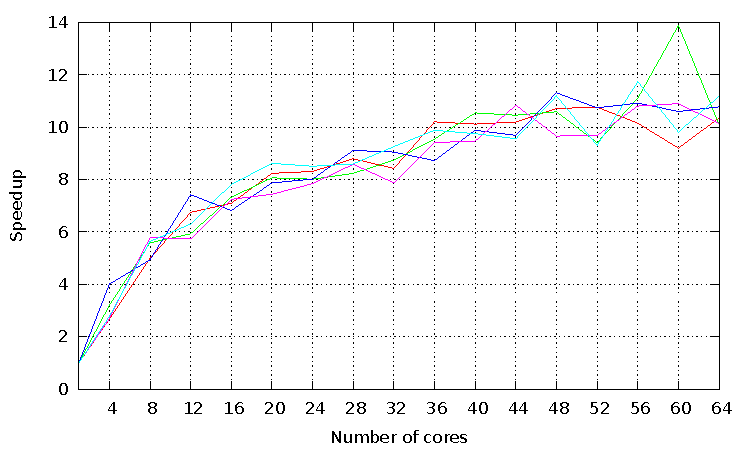
\includegraphics[width=0.9\textwidth]{parallel_speedup.pdf}
    \caption{Speedup of embarrasingly parallel program (5 runs)}
    \label{fig:parallel_speedup}
\end{figure}

This experimental data shows that Erlang can be used for many-core programs,
but, like we see from work by Jianrong\cite{erlang-manycore-scalability}, VM
needs tuning in order to achieve significant linear scalability.

Currently in Erlang message sending between processes is implemented using
shared memory, locks and mutexes. However, it would be a very interesting
project to replace inter-erlang-process communication with UDN eliminating the
need of shared memory at all. Most importantly, application developer would not
notice the usability change at all; however, this would potentially eliminate
shared memory bottleneck.

\section{Further topics}

\clearpage
\begin{thebibliography}{99}

    \bibitem{fggc} Sutra,~P. \emph{Fast Genuine Generalized Consensus}. Reliable
        Distributed Systems (SRDS), 2011 30th IEEE Symposium.

    \bibitem{hipe} Sagonas,~K., Wilhelmsson,~J. \emph{Efficient memory
        management for concurrent programs that use message passing}. Science of
        Computer Programming, 62(2): p.~98-121, October 2006.

    \bibitem{1kcorechips} Borkar,~S. \emph{Thousand Core Chips—A Technology
        Perspective}. DAC '07 Proceedings of the 44th annual Design Automation
        Conference. p.~746-749.

    \bibitem{pollack} Pollack,~F. \emph{Pollack's Rule of Thumb for
        Microprocessor Performance and Area.}

    \bibitem{future-microprocessors} Borkar~S., Chien,~ A.~A. \emph{The Future
        of Microprocessors}. Communications of the ACM, Vol. 54 No. 5, p.~67-77.

    \bibitem{tile64} Bell,~S., Edwards,~B., Amann,~J., Conlin,~R.,
        Joyce,~K., Leung,~V., MacKay,~J., Reif,~M., Bao,~L., Brown,~J.,
        Mattina,~M., Miao,~Chyi-Chang, Ramey,~C., Wentzlaff,~D.,
        Anderson,~W., Berger,~E., Fairbanks,~N., Khan,~D., Montenegro,~F.,
        Stickney,~J., Zook,~J. \emph{TILE64 -- Processor: A 64-Core SoC with
        Mesh Interconnect}. Solid-State Circuits Conference, 2008. ISSCC 2008.
        Digest of Technical Papers. IEEE International. p.~88-598.

    \bibitem{classic-paxos} Lamport,~L. \emph{The part-time parliament}. ACM
        Transactions on Computer Systems (TOCS). Volume 16 Issue 2, May~1998.
        p.~133-169.

    \bibitem{paxos-simple} Lamport.,~L. \emph{Paxos made simple}. ACM SIGACT
        News (Distributed Computing Column) 32, 4 (Whole Number 121, December
        2001) p.~51-58.

    \bibitem{generalized-consensus} Lamport.~L. \emph{Generalized Consensus and
        Paxos}. Microsoft Research Technical Report MSR-TR-2005-33.

    \bibitem{chubby} Burrows,~M. \emph{The Chubby lock service for
        loosely-coupled distributed systems}. OSDI '06 Proceedings of the 7th
        symposium on Operating systems design and implementation. p. 335-350.

    \bibitem{openreplica} Altinbuken,~D., Emin~Gun.,~S. \emph{Commodifying
        Replicated State Machines with OpenReplica}. Computing and
        Information Science Technical Reports, Cornell University.

    \bibitem{erlang-acoustic} Convey,~C., Fredricks,~A., Gagner,~C.,
        Maxwell,~D., Hamel,~L. \emph{Experience report: erlang in acoustic ray
        tracing}. In ICFP ’08: Proceeding of the 13th ACM SIGPLAN international
        conference on Functional programming, pages 115–118, New York, NY, USA,
        2008. ACM.

    \bibitem{vm-manycore} Marr,~S. D’Hondt,~T. \emph{Many-core virtual machines:
        decoupling abstract from concrete concurrency}. In SPLASH ’10:
        Proceedings of the ACM interna- tional conference companion on Object
        oriented programming systems languages and applications companion.
        p.~239–240, New York, NY, USA, 2010. ACM.

    \bibitem{erlang-manycore-scalability} Jianrong, Z. \emph{Characterizing the
        Scalability of Erlang VM on Many-core Processors}. Student thesis, KTH,
        School of Information and Communication Technology (ICT).

\end{thebibliography}
\end{document}
